\documentclass{article}
\usepackage{fullpage}
\usepackage{lastpage}
\usepackage{fancyhdr}
\usepackage{amssymb}
\usepackage{amsmath}
\usepackage{graphicx,subcaption} 
\usepackage{mathtools}
\usepackage{enumerate}
\usepackage{xspace}
\usepackage{txfonts}
\begin{document}
\begin{center}
{\Large \textbf{CMPUT 656 Course Project: Learning What to Remember}}
\end{center}
\section*{Introduction}
Most reinforcement learning techniques assume the environment has the Markov property, meaning that the future state is independent of the past states give the present states. Put another way this assumes the agent has all the information it needs to make an optimal decision at each time and therefore has no need to remember the past. This is however not realistic in general, realistic problems often require significant information from the past in order to make an informed decision in the present and there is often no obvious way to incorporate the relevant information into an expanded present state. It is therefore desirable to establish general techniques for learning a compact representation of the relevant details of the past (i.e. a memory, or learned state) in order to facilitate decisions in the present.
Most modern attempts to tackle this problem make use of variations of recurrent neural networks trained with back-propagation through time. This can work well for many tasks, but generally requires backpropogating many steps into the past which is not practical in an online reinforcement learning setting. In this work we attempt to address the problem of memory without explicit backpropogation through time. To do this we propose a method for learning over time which information should be written to and read from a lossy external memory. If an RNN can be considered a working memory

\section*{Problem}
As a proof of concept for our proposed method we propose a toy problem we call "the secret informant" problem which requires an agent to figure out what information from past states is informative about the correct decision to make in the future. The environment consists of a chain of states each represented by a feature vector. In each state k possible actions are available (we use k=3 throughout), however the action choice only changes the outcome in the final state where 1 of the three actions will yield a reward of $+1$ and the other 2 will yield $0$ reward. Which action will yield the reward is drawn uniformly for each episode of the problem and can be determined for a given episode only by looking at the feature vector of some past state (which we refer to as the informant state) prior to the state in which the choice must be made. The feature vector associated with each state is shown in figure \ref{fig:state}.

The agent starts with no knowledge of the semantic interpretation of the state representation and must learn through successive trials what information is relevant to allow it to select the correct action in the final state. It also does not initially know that reward is only available in the final state and all other actions are irrelevant so this too must be learned. An instance of the full problem is shown in \ref{fig:problem}.
\begin{figure}[!ht]
\center
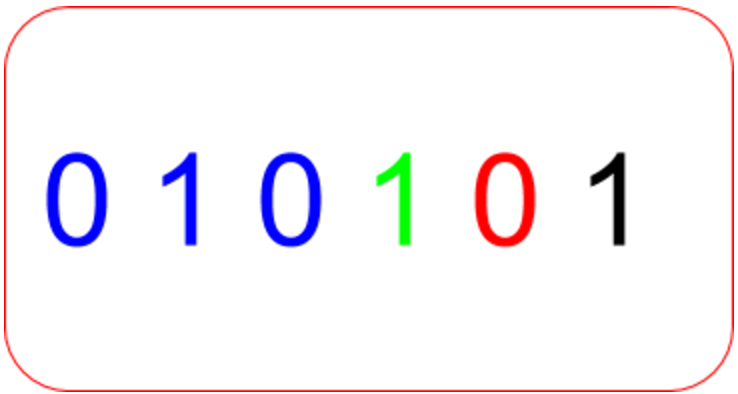
\includegraphics[width=0.5\textwidth]{images/state.png}
\caption{State representation for our test problem, blue digits are a one hot representation of which action the state is suggesting is correct (i.e. will yield $+1$ reward), the green digit will be 1 if and only if this state actually determines the correct action to take (i.e. it is the informant state). The red digit will be 1 if and only if the blue indicator is random and uncorrelated with the correct action choice (i.e. it is a noisy state). The final digit is simply an always on bias which may aid in the memory mechanism we will describe later. In addition to the general interpretation of these digits there is a special start node with code 000001 and the final node (at which the action choice will give a reward) with code 000011.}
\label{fig:state}
\end{figure}

\begin{figure}[!ht]
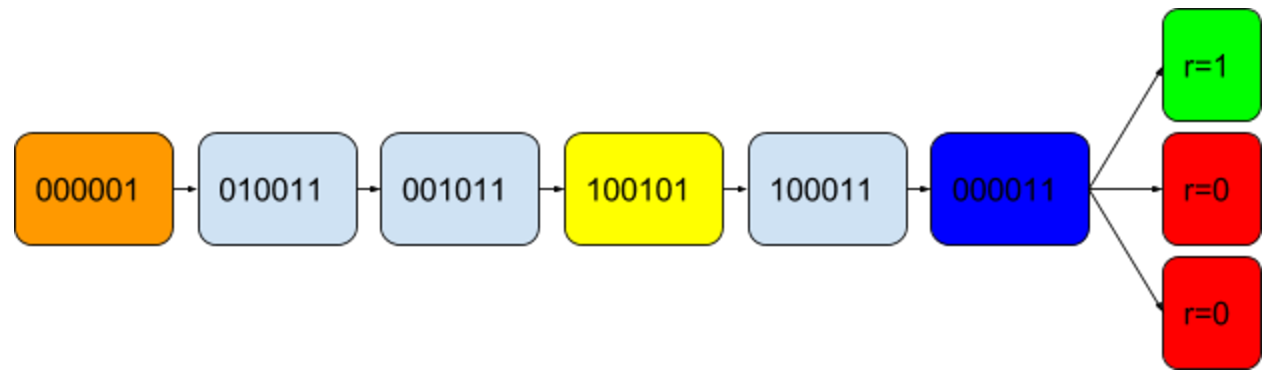
\includegraphics[width=1\textwidth]{images/problem.png}
\caption{An instance of the secret informant, the start state is orange, the final state (at which a decision must be made) is dark blue, the informant state (with the 4th bit set to 1) is yellow while the noisy states (with the 4th bit set to 0) are pale blue. Notice that because the 1st bit in the informant state is 1 and the rest are 0 the reward must be given for the top action and no other. In each instance of the problem the informant state will be placed randomly between the start and final state. Here we have 3 noisy states in addition to the informant state, in our tests we use 4 noisy states.}
\label{fig:problem}
\end{figure}

\section*{Related Work}

\section*{Proposed Method}
The main contribution of this work is to suggest a new kind of memory module designed to be trainable to both read and write using only information local in time (i.e. without requiring something like backpropagation through time). The instantiation of this idea presented here is meant only as a proof of concept with much room for improvement in terms of both theoretical foundation and actual implementation.
\subsection*{Memory Module}
The memory module is inspired by (though currently quite different from) the Holographic Reduced Representation used in \cite{LSTM}, and is intended to store and recall vectors of a fixed length $n$. It consists of $m$ complex copies, each of length $n$. Each time a write is performed it is accompanied by a positive weight $r$ (fixed here to be in $[0,1]$) which simply multiplies the item to be stored and corresponds to how strongly we wish to remember the current state. Additionally each copy is multiplied by a uniformly random complex phase $e^{i\theta_k}$ chosen separately for each copy stored. If we take the memory to be an $(m,n)$ complex matrix $M$ writing a vector $\pmb{s}$ with weight $r$ is done as follows:

$$M_{k,j}\mathrel{+}=re^{i\theta_k}\pmb{s}_j$$

Where here $j$ indexes the elements of the stored vector $\pmb{s}$ and $k$ indexes the $m$ copies stored in the memory. Now consider how we can go about recalling stored items from this memory. If we knew the set of random phases with which the desired item was stored $e^{i\theta_k}$ we can multiply each copy by its complex conjugate $e^{-i\theta_k}$ and take the real part of the result to retrieve an estimate $\tilde{\pmb{s}}_k$ of $\pmb{s}$. Since the phases used for all other stored items are uniformly random they will still be uniformly random when multiplied by $e^{-i\theta_k}$. i.e. for a particular $k$ and $\pmb{s_t}$ where $t$ is the time-step we wish to recover our written value from, we get an estimate that looks like this:
\begin{align*}
\tilde{\pmb{s_t}}_{k}&=\Re(e^{-i\theta_{kt}}M_{k,:})\\
&=\Re(r_t\pmb{s_t}+\sum_{\tau\neq t}e^{i(\theta_{k\tau}-\theta_{kt})}r_\tau\pmb{s_\tau})\\
&=r_t\pmb{s_t}+\Re(\sum_{\tau\neq t}e^{i(\theta_{k\tau}-\theta_{kt})}r_\tau\pmb{s_\tau})\\
&=r_t\pmb{s_t}+(\textit{Expectation 0 Noise})
\end{align*}
By Averaging the resulting estimates $\tilde{\pmb{s_t}}_{k}$ over all $m$ copies in memory we get a better unbias estimate of $r_t\pmb{s_t}$. In order to get rid of the scaling factor $r_t$ we enforce that all the $\pmb{s_t}$ are normalized before being written to memory, thus we simply normalize the resulting estimate of $r_t\pmb{s_t}$ to obtain an estimate of $\pmb{s_t}$ itself.

The bad news is we do not actually know the complex phases $e^{-i\theta_k}$ for the particular item we are trying to recall. The only information we are storing is the $m$ complex vectors that make up the memory. In the present work we use a particular method for querying the memory and estimating these phases, however the theoretical details have not been fully hashed out. Refining our memory mechanism to have better understood theoretical properties (which hopefully translates into better results and greater applicability) is a task for future work.

The way we handle queries to the memory is a form of content addressable read mechanism. A query to the memory consists of an arbitrary real vector of length $n$ (the same as the length of the stored items). For each copy in the memory we then estimate the phase of the desired read value to be the phase which results in the maximum dot product between the query $\pmb{q}$ and the returned estimate $\tilde{\pmb{s_t}}_{k}$. As we will now show this maximization process is a differentiable operation and can thus be trained by backpropagation directly.
\begin{align*}
\theta_k&=\underset{\theta}{argmax}\  \Re(e^{i\theta}\pmb{q}\cdot M_{k,:})\\
&=\underset{\theta}{argmax}\  \Re(\cos(\theta)\pmb{q}\cdot M_{k,:}+i\sin(\theta)\pmb{q}\cdot M_{k,:}\\
&=\underset{\theta}{argmax}\  \cos(\theta)\Re(\pmb{q}\cdot M_{k,:})-\sin(\theta)\Im(\pmb{q}\cdot M_{k,:})\\
&\implies \frac{d}{d\theta}\left(\cos(\theta)\Re(\pmb{q}\cdot M_{k,:})-\sin(\theta)\Im(\pmb{q}\cdot M_{k,:})\right)=0\text{, at }\theta_k\\
&\implies -\sin(\theta_k)\Re(\pmb{q}\cdot M_{k,:})-\cos(\theta_k)\Im(\pmb{q}\cdot M_{k,:})=0\\
&\implies \tan(\theta_k)=-\frac{\Im(\pmb{q}\cdot M_{k,:})}{\Re(\pmb{q}\cdot M_{k,:})}\\
&\implies \theta_k=n\pi-\arctan\left(\frac{\Im(\pmb{q}\cdot M_{k,:})}{\Re(\pmb{q}\cdot M_{k,:})}\right)\text{, for some integer }n
\end{align*}
Note that angles differing by $2\pi$ are equivalent hence there are really 2 extrema here, one is a minimum and one is a maxima. To figure out which is which we can look at the second derivative. After doing this and performing some simple algebra we find that the maxima we desire is given by:
$$\theta_k = \begin{cases}
 -\arctan\left(\frac{\Im(\pmb{q}\cdot M_{k,:})}{\Re(\pmb{q}\cdot M_{k,:})}\right) &\text{if $\Re(\pmb{q}\cdot M_{k,:})\geq0$}\\    \pi-\arctan\left(\frac{\Im(\pmb{q}\cdot M_{k,:})}{\Re(\pmb{q}\cdot M_{k,:})}\right) &\text{if $\Re(\pmb{q}\cdot M_{k,:})<0$}
\end{cases}
$$
We can use this angle to find the estimated $\pmb{s}$ in memory ``closest'' to the query $\pmb{q}$ as described above. Note that since this optimal angle and the subsequent computation of the estimate $\pmb{s}$ described above are both differentiable almost everywhere, we can backpropogate through this to improve our generated queries $\pmb{q}$ in order to make use of our stored memories to achieve our specified task.

\subsection*{Training Write Network}
As highlighted above the query portion of our network is fully differentiable and therefore trainable directly by backpropogation. In addition we have a second network whose purpose is to choose the write weight $r$ for the state at each time-step. While in principle the right portion of the network is also differentiable and could also be trained by a variant of backpropogation through time, the purpose of the present work is to design a method which avoids this, thus we instead use an update method which is strictly local in time. Our method attempts to approximate $\frac{d\sigma^2(Q(\pmb{s},a))}{dr(\pmb{q})}$ (i.e. the change in the variance of each action value in the current state over the change in the write weight associated with the current query). Using this estimate we then compute $\frac{d\sigma^2(Q(\pmb{s},a))}{\theta}=\frac{d\sigma^2(Q(\pmb{s},a))}{dr(\pmb{q})}\frac{dr(\pmb{q})}{\theta}$ for each parameter $\theta$ of the write network. This value is then used to perform gradient descent to tune the write network to generate weights which produce low variance in the computed action values.
\subsection*{Architecture}
\begin{figure}[!ht]
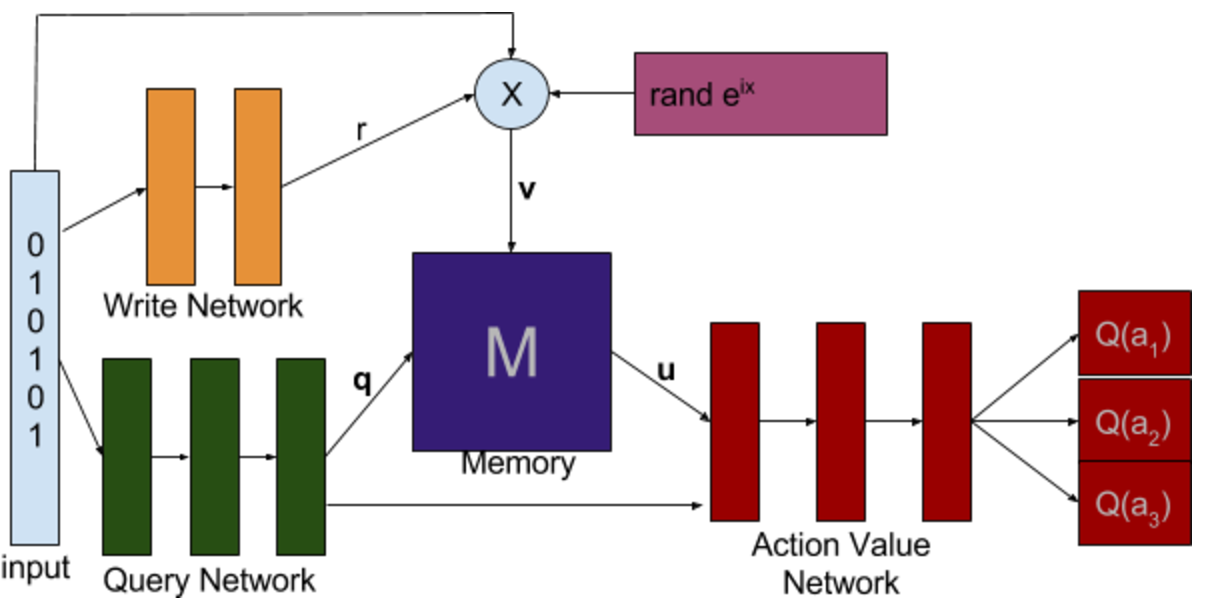
\includegraphics[width=1\textwidth]{images/architecture.png}
\caption{Our architecture, input is given separately to both query and write network. Write network output is sigmoid to give a weight between 0 and 1, this weight multiplies the input vector input along with a random complex phase to give the value that is actually written to memory. The query network output \textbf{q} to memory is identity (i.e. potentially spans the whole space) the memory returns a vector \textbf{u}. The input to the action value network consists of the output of the second last layer of the query network, along with the value \textbf{u} read from memory. The action value network outputs action values for all available actions.  }
\label{fig:arch}
\end{figure}

\section*{Results}
\begin{figure}[!ht]
\centering
\begin{subfigure}[t]{.45\textwidth}
  \centering
      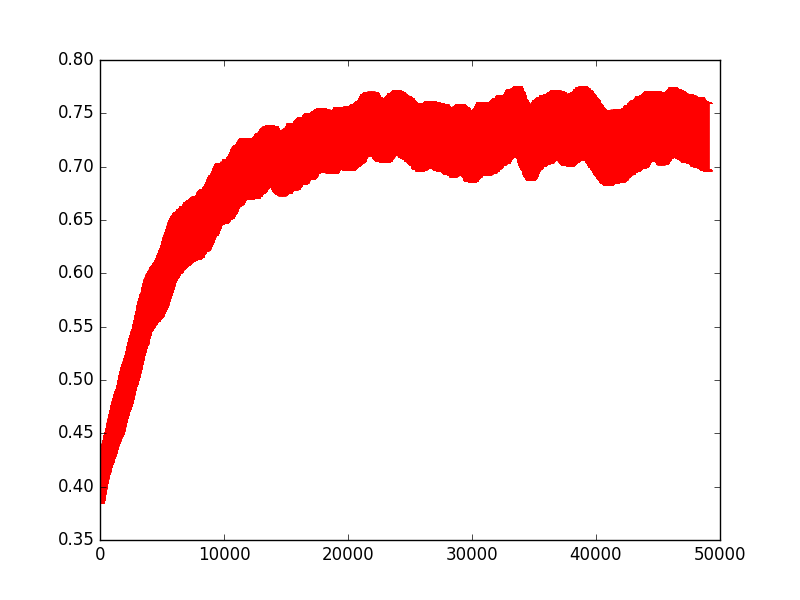
\includegraphics[width=1\textwidth]{images/1_query_mem_ret.png}
  \caption{Returns over time for 1 query architecture. y-axis is return, x-axis is number of training episodes.}
  \label{fig:1_query_ret}
\end{subfigure}\hfill
\begin{subfigure}[t]{.45\textwidth}
  \centering
      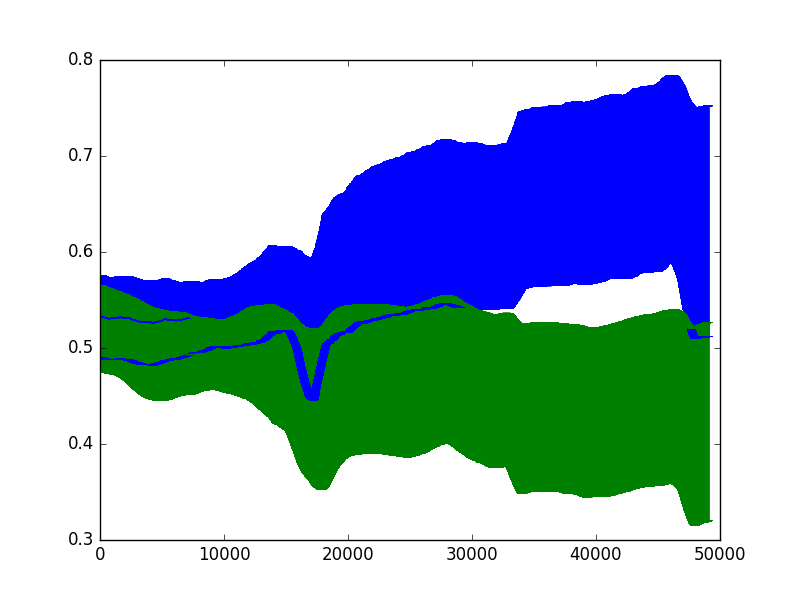
\includegraphics[width=1\textwidth]{images/1_query_mem_writes.png}
  \caption{Write weight for informant state (blue) and average write weight for all other states (green). y-axis is write weight, x-axis is number of training episodes.}
  \label{fig:1_query_write}
\end{subfigure}
\caption{Results for architecture with 1 query}
\label{fig:1_query}
\end{figure}

\begin{figure}[!ht]
\center
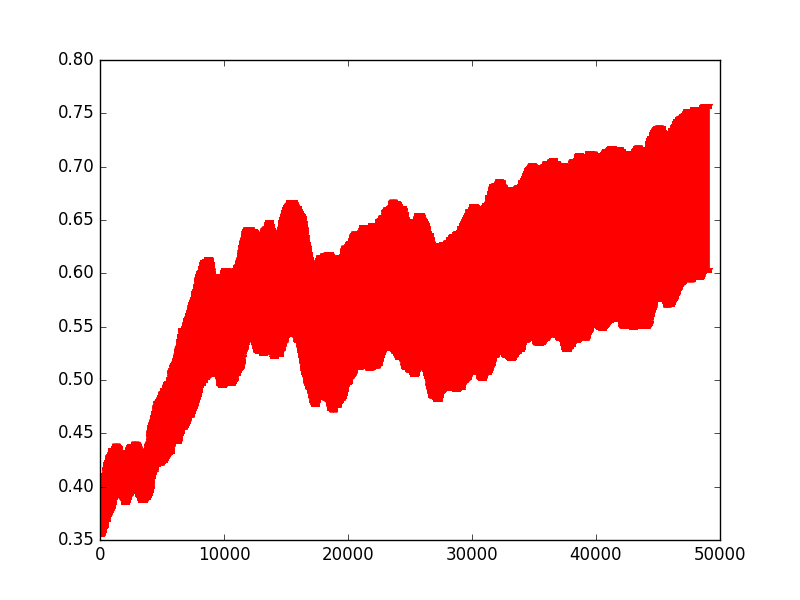
\includegraphics[width=0.5\textwidth]{images/1_query_mem_ret_no_write.png}
\caption{Returns over time for 1 query architecture but with write weight fixed to 1 for all time steps. y-axis is return, x-axis is number of training episodes. This is not exactly conclusive but comparing to Figure \ref{fig:1_query_ret} it does appear that using write weight tuning helps to improve the return faster.}
\label{fig:1_query_no_write}
\end{figure}

\begin{figure}[!ht]
\centering
\begin{subfigure}[t]{.45\textwidth}
  \centering
      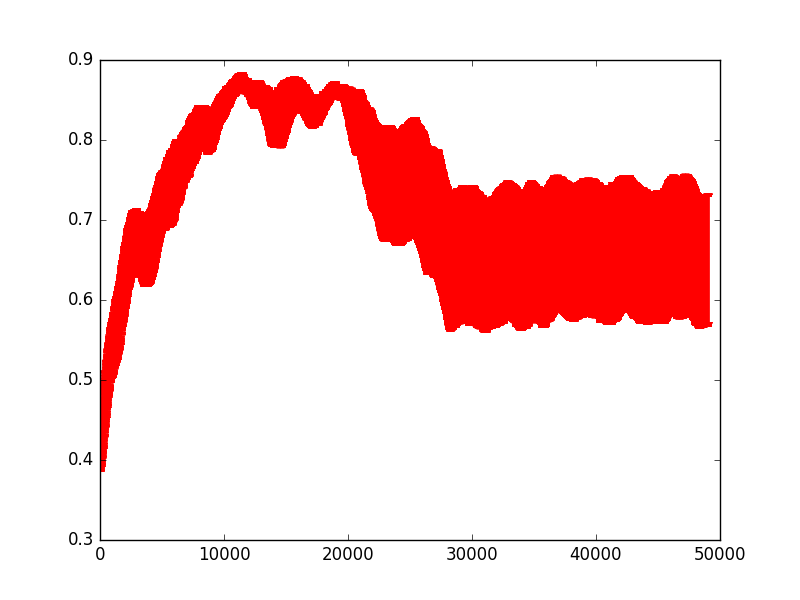
\includegraphics[width=1\textwidth]{images/5_query_mem_ret.png}
  \caption{Returns over time for 5 query architecture. y-axis is return, x-axis is number of training episodes.}
  \label{fig:5_query_ret}
\end{subfigure}\hfill
\begin{subfigure}[t]{.45\textwidth}
  \centering
      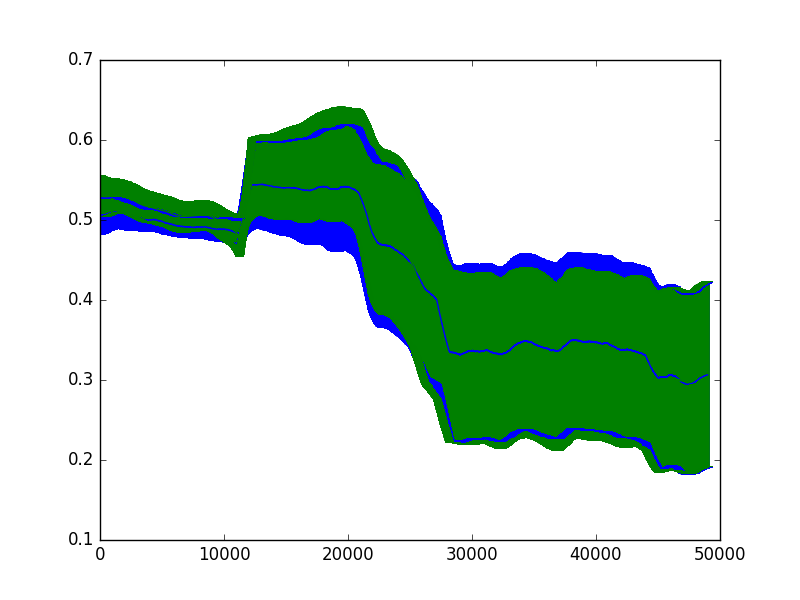
\includegraphics[width=1\textwidth]{images/5_query_mem_writes.png}
  \caption{Write weight for informant state (blue) and average write weight for all other states (green). y-axis is write weight, x-axis is number of training episodes.}
  \label{fig:5_query_write}
\end{subfigure}
\caption{Results for architecture with 5 queries. Initial improvement in return is more rapid and consistent, however it collapses somewhat later on. Additionally the write weights don't appear to separate at all as they did in the 1 query case. }
\label{fig:5_query}
\end{figure}

\begin{figure}[!ht]
\center
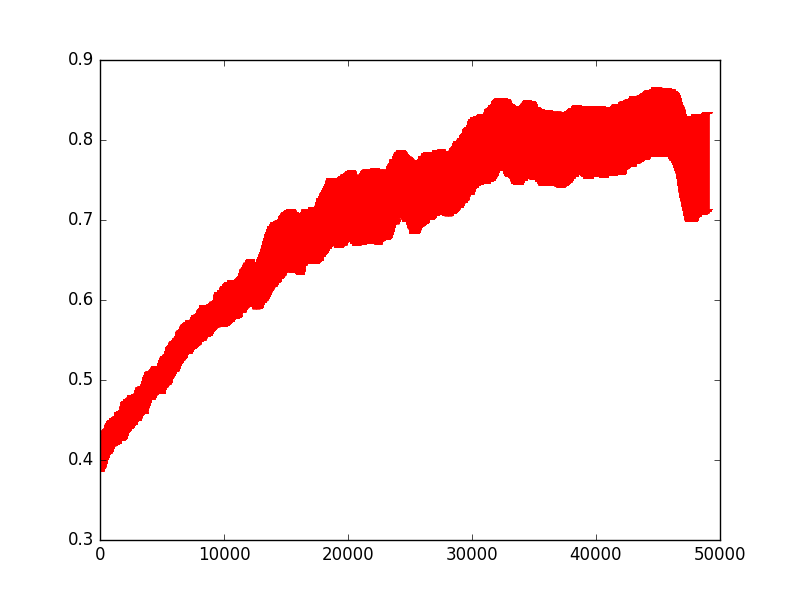
\includegraphics[width=0.5\textwidth]{images/recurrent_ret.png}
\caption{Returns over time for recurrent baseline. y-axis is return, x-axis is number of training episodes.}
\label{fig:recurrent}
\end{figure}

\section*{Discussion}

\section*{Conclusion}

\section*{Future Work}


\begin{thebibliography}{plain}
\bibitem{NTM}
Graves, A., Wayne, G., and Danihelka, I. (2014) Neural Turing Machines. arXiv preprint arXiv:1410.5401.

\bibitem{MC}
Oh, J., Chockalingam, V., Singh, S., and Lee, H. (2016) Control of Memory, Active Perception, and Action in Minecraft. ICML, New York City, 2016. JMLR Workshop and Conference Proceedings Volume 48.

\bibitem{LSTM}
Danihelka, I., Wayne, G., Uria, B., Kalchbrenner, N., and Graves, A. (2016) Associative Long Short-Term Memory. ICML, New York City, 2016. JMLR Workshop and Conference Proceedings Volume 48.

\bibitem{DNC}
Graves, A. et al. (2016) Hybrid Computing Using a Neural Network with Dynamic External Memory. Nature 538, 471-476.
\end{thebibliography}



\end{document}